% Overview figure (fig:overview). Build (from report/final_en): cd figures_front && FONTCONFIG_FILE=../fontconfig/fonts.conf xelatex overview.tex -> overview.pdf
% Numbers: juliet/full_split_v1.json (1,658 groups, 3,316 units) and juliet_full/data/README.md.
\documentclass[tikz,border=1pt]{standalone}
\usepackage{fontspec}
\setmainfont{TeX Gyre Termes}
\setsansfont{TeX Gyre Heros}
\setmonofont{TeX Gyre Cursor}
\usetikzlibrary{positioning,arrows.meta,fit,calc}
\begin{document}
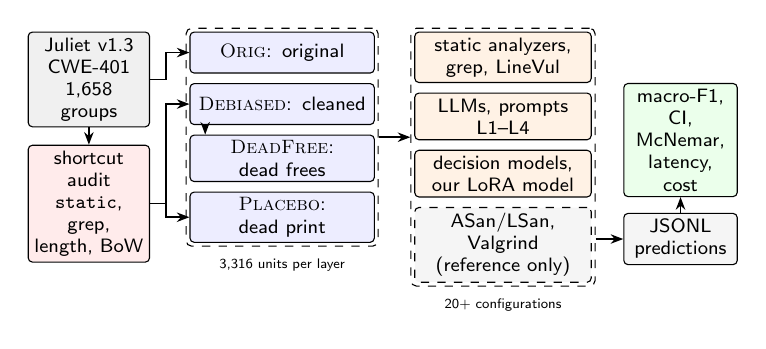
\begin{tikzpicture}[
  font=\sffamily\scriptsize,
  node distance=2.2mm and 3mm,
  box/.style={draw, rounded corners=1.5pt, align=center, inner sep=2pt, minimum height=6.5mm},
  src/.style={box, fill=gray!12, text width=14mm},
  layer/.style={box, fill=blue!7, text width=22mm, minimum height=5.2mm},
  det/.style={box, fill=orange!10, text width=21mm, minimum height=5.2mm},
  arr/.style={-{Stealth[length=1.6mm]}, semithick},
]
% column 1: source and audit
\node[src] (juliet) {Juliet v1.3\\ CWE-401\\ 1,658 groups};
\node[src, below=of juliet, fill=red!8] (audit) {shortcut audit\\ \texttt{static}, grep,\\ length, BoW};
% column 2: benchmark layers
\node[layer, right=5mm of juliet.north east, anchor=north west] (orig) {\textsc{Orig}: original};
\node[layer, below=1.2mm of orig] (deb) {\textsc{Debiased}: cleaned};
\node[layer, below=1.2mm of deb] (dead) {\textsc{DeadFree}: dead frees};
\node[layer, below=1.2mm of dead] (plac) {\textsc{Placebo}: dead print};
% column 3: detectors
\node[det, right=5mm of orig.north east, anchor=north west] (stat) {static analyzers,\\ grep, LineVul};
\node[det, below=1.2mm of stat] (llm) {LLMs, prompts L1--L4};
\node[det, below=1.2mm of llm] (dm) {decision models,\\ our LoRA model};
\node[det, below=1.2mm of dm, fill=gray!8, dashed] (dyn) {ASan/LSan, Valgrind\\ (reference only)};
% column 4: metrics
\node[box, fill=green!8, text width=13mm, right=4mm of llm.east, anchor=west, yshift=-3mm] (met) {macro-F1,\\ CI, McNemar,\\ latency,\\ cost};
\node[box, fill=gray!8, text width=13mm, below=2mm of met] (run) {JSONL\\ predictions};
% arrows
\draw[arr] (juliet) -- (audit);
\draw[arr] (juliet.east) -- ++(2mm,0) |- (orig.west);
\draw[arr] (audit.east) -- ++(2mm,0) |- (deb.west);
\draw[arr] ($(deb.south west)+(2mm,0)$) -- ($(dead.north west)+(2mm,0)$);
\draw[arr] ($(audit.east)+(2mm,0)$) |- (plac.west);
\node[draw, dashed, rounded corners=2pt, inner sep=1.2pt, fit=(orig)(plac)] (L) {};
\node[draw, dashed, rounded corners=2pt, inner sep=1.2pt, fit=(stat)(dyn)] (D) {};
\draw[arr] (L.east) -- (L.east -| D.west);
\draw[arr] (D.east |- run) -- (run.west);
\draw[arr] (run) -- (met);
\node[below=0.3mm of L.south, font=\sffamily\tiny] {3,316 units per layer};
\node[below=0.3mm of D.south, font=\sffamily\tiny] {20+ configurations};
\end{tikzpicture}
\end{document}
